% preprint draft due June 14
% final draft due July 27

% TUGboat class documentation is at:
%   texdoc tugboat
% or
%   https://texdoc.org/serve/tugboat/0
% or
%   https://mirrors.ctan.org/macros/latex/contrib/tugboat/ltubguid.pdf

% guidelines: https://tug.org/TUGboat/location.html

% here's how I made a Calculus book accessible
% Ulrike Fischer: Showing a real, large document
% (perhaps including some remarks how well accessibility works and what
% doesn't work) sounds interesting.
% And showing that "normal" users can actually do that if they try
% is an important message.

% keep source lines to <= 79 characters
%234567891_234567892_234567893_234567894_234567895_234567896_234567897_23456789

% messes up the verbatim blocks
%\DocumentMetadata{
%  lang=en,
%  tagging=on,
%  pdfstandard=ua-2,
%%  check-tagging-status,
%  tagging-setup={
%%    math/alt/use,
%    math/setup=mathml-SE
%  }
%}

\documentclass{ltugboat}
\usepackage{graphicx}
\usepackage{tikz-cd}
\usepackage{unicode-math}
\usepackage{amsmath}
\usepackage{pgfplots}
\usepackage{booktabs}
\usepackage{siunitx}
\usepackage{microtype}
\usepackage[normalem]{ulem}
%\usepackage{xurl}
\usepackage[hidelinks]{hyperref}

\def\url{\tburl}

\IfDocumentMetadataF{
 \pgfqkeys{/tikz}{alt/.code={}}
}
\newcommand{\verbatimoptions}{%
 \IfDocumentMetadataT{setup-code=}\small\makevmeta
}

\newcommand{\veraPDF}{vera\PDF}
\newcommand{\VeraPDF}{vera\PDF}  % it appears they are always lower case
\newcommand{\PDFix}{\PDF ix}

\DeclareMathOperator{\coker}{coker}
\pgfplotsset{compat=1.18}

\title{Converting a \PDF\ textbook to be accessible}

\addtolength{\signaturewidth}{25pt}
\author{Timothy Prescott}
%\address{University of North Dakota\\101 Cornell Street Stop 8376\\
%Grand Forks ND, 58203\\ USA}
\netaddress{timothy dot prescott (at) UND dot edu}
%\personalURL{https://und.edu/directory/timothy.prescott}
%\ORCID{0009-0009-0555-8074}

% electronic access to the TUGboat issue suffices

\begin{document}
\maketitle

\begin{abstract}
A guideline in the United States requires that
\PDF s created after April 2026 must be accessible
to visually impaired users.
We discuss
how we updated a custom three semester calculus book to be accessible,
including what we did, the challenges we faced,
how we verified accessibility, and what remains to be done.
We also discuss
% creating accessible \texttt{beamer} style presentations
% using \texttt{ltx-talk}, and
necessary adaptations
to satisfy a common accessibility checker available in several \acro{LMS}s.
\end{abstract}

\section{Introduction \& setup}

Since 2016, the University of North Dakota has used
a custom 1150 page textbook for its three semester calculus sequence.
The source for the textbook is at
\cite{ApexURL},
%\url{https://github.com/teepeemm/APEXCalculusLT_Source},
forked from
%\url{https://github.com/APEXCalculus/APEXCalculus_Source},
\cite{Hartman},
while the compiled document is at
\cite{ApexUNDurl}.
%\url{https://arts-sciences.und.edu/academics/math/calc-1-texts.html}.

Using a custom textbook has enabled students
to download the \PDF\ for free
in addition to having the option to purchase the book
for a fraction of the cost of other textbooks
(currently \$25--\$30 per semester, when I last checked).

The format of the book is to \cs{include} one \cs{part} for each semester,
so that \cs{includeonly} allows us to have three one semester \PDF s that we
send to the university printer to create physical copies
(the online \PDF\ includes all three semesters).
Within each included file, there are a few paragraphs introducing each chapter
and we then \cs{input} each section.
Each section then ends with a custom command that inputs the exercises
for that section.

My university has been emphasizing the national requirement
that all documents must satisfy the \acro{WCAG 2.1 AA} guideline
as of April 2026 (now delayed to 2027); see \TUB\ 45:2 \cite{Kuan:2024:LCL}
for a historical overview of how we got to this point.
Beginning in early 2025, I began exploring how to ensure that
the textbook meets this guideline.

\section{The basics}

My starting point for \LaTeX\ accessibility is
\cite{taggingStartPoint}.
%\url{https://latex3.github.io/tagging-project/documentation/prototype-usage-instructions.html}.
I first needed to convert the document from using \XeLaTeX\ to \LuaLaTeX,
which also necessitated adjusting a few font commands in the preamble,
but not much else.

The \LaTeX\ team has reported their progress developing tagging
since at least \TUB\ 40:2 \cite{Rowley:2019:ALK}
(see also \cite{tugKeywordAccessible}),
%\url{https://tug.org/TUGboat/Contents/listkeyword.html#CatTAGAccessibility}
building off of existing efforts.
% should I cite others from TUGboat?
Thanks to their hard work,
the vast majority of accessibility is enabled by using
%\begin {verbatim}
%\begin{verbatim}[setup-code=\small]
\begin{verbatim}[\verbatimoptions]
\DocumentMetadata{
  lang=en,
  tagging=on,
  pdfstandard=ua-2,
%  check-tagging-status,
  tagging-setup={
%    math/alt/use,
    math/setup=mathml-SE } }
\documentclass{...}
\usepackage{unicode-math}
\end{verbatim}
as the first commands of the document.
I'll discuss the commented options as we proceed;
other options are available by looking through
\texttt{texdoc documentmetadata-support-code}.
In addition to enabling tagging, the \cs{DocumentMetadata} command
can adjust the \PDF\ metadata of the compiled document.

An all too common occurrence during compilation was a tagging related error,
often that ``The number of automatic begin and end hooks differ!''
My setup of using \cs{include} and \cs{input} allowed me to comment out
various sections, isolating a single section that caused the error.
I then examined the log file,
found a ``Package tagpdf Warning'' regarding some aspect of the code, and
created a minimal working example causing this warning and error.

With the example in hand, I began searching the internet for a fix.
For packages, a good starting point was to view
\cite{taggingStatus},
%\url{https://latex3.github.io/tagging-project/tagging-status/},
which reports the tagging compatibility of each class and package.
Often, a linked issue contained code snippets I copied and pasted
into the preamble that resolved the issue.

Uncommenting the \texttt{check-tagging-status} line
in the \cs{DocumentMetadata} will also create
a tagging status report in the log file.
The \texttt{tagging-status} website and log information have five categories:
\begin{description}
\item[compatible] Everything should work for the package, and
 the \LaTeX\ team wants to know if it doesn't.
 This is the most common entry for the website.
\item[partially-compatible] The package should work
if you avoid issues described in the website.
\item[currently-incompatible] Double check the issue(s) in the website
to see if you can make it work.
\item[no-support / unsupported] You need to find a new package%
\footnote{If a package in this category
is causing errors because you use \cs{DocumentMetadata} solely
to adjust the \PDF\ metadata,
you can use the \texttt{pdfmanagement} package
instead of \cs{DocumentMetadata}}.
\item[unchecked / unknown / unclassified] The package has not been tested.
Your odds are good if some other package loaded it;
your odds are bad if it's a local package provided by a ``friend''.
%good luck / who knows / may the force be with you / YMMV
\end{description}

Resolving errors not directly related to packages was more difficult.
I often turned to the \TeX\ Stack
Exchange\footnote{\url{https://tex.stackexchange.com/}} for help.
(In more extreme cases,
I reported a bug to the tagging project's GitHub
repository\footnote{\url{https://github.com/latex3/tagging-project}}.
Luckily for the reader (and the author), some errors were caused
by a bug in the tagging code that was quickly fixed.
(A quickly fixed bug was also occasionally true
of errors relating to packages.)

How much time you'll need to spend getting through this step depends on
how much the existing document follows some general guidelines:
\begin{itemize}
\item Use modern, best practices \LaTeX.
(That code that has always produced the desired \PDF\ even though
people looking at have said ``that's not the right way to do it''?
Now is the time to get better code.)
\item Further, aim for a clean log file.
The tagging software writes useful information to the log file
that is difficult to find if it's full of warnings
(you're not ignoring error messages, are you?).
\item Arrange your code so that the content is in the \tubbraced{document},
while the preamble takes care of the formatting, style, and execution.
\item For example, make liberal use of \tubbraced{environments}.
Environments make it clearer where a portion of the \PDF\ should begin and end.
They also automatically provide several useful points where you can hook code.
\end{itemize}

\section{Alt text}

With \LuaLaTeX\ automatically handling the bulk of the work,
the greatest part of the work requiring manual intervention was
providing alternative text for the thousand images throughout the book.
Alt text provides a verbal description of an image
that a visually impaired person has difficulty seeing.
Ideally, alt text should be
\begin{itemize}
\item brief (at most 120 characters or 2 sentences)
\item objective
\item not the sole source of necessary information
(most users will not see the alt text)
\item not begin with the word ``image'',
so that a screen reader does not say ``Image: image \dots''
\item not blindly copied from an AI output
\end{itemize}
A guideline I often tell myself is
``How would I tell someone to sketch this image?''

\LaTeX's tagging code can specify alt text as an optional argument
to the image:
\begin{itemize}
\ttfamily
\item\cs{includegraphics}[\textbf{alt=\tubbraced{...}}]
\item\cs{tikz}[\textbf{alt=\tubbraced{...}}]
\item\cs{begin}\tubbraced{tikzpicture}[\textbf{alt=\tubbraced{...}}]
\item\cs{begin}\tubbraced{picture}[\textbf{alt=\tubbraced{...}}]
\end{itemize}
There are also two substitutes to \texttt{alt=\tubbraced{...}}:
we can use the option \texttt{artifact}
if the image is purely decorative and unnecessary for the reader,
so that screen readers ignore it entirely.
Less commonly, we can use \texttt{actualtext=\tubbraced{...}}
so that screen readers act as if there is no image,
and instead read the text.
This works best if the image is actually stylistically decorated text.

It is useful to note that creating alt text is
the least \TeX nical aspect of this article.
A majority of this discussion requires some experience with creating
a longer \LaTeX\ document.
For alt text, however, I used a short Python script that added
\texttt{alt=\tubbraced{ALT-TEXT-TO-BE-DETERMINED}} to all of the images.
A student worker with less \TeX\ experience was then able to go through
the book, examine the resulting \PDF, and create the alt text.

\subsection{Issues related to alt text}

There are two contrasting problems arising from alt text.
The first was succinctly stated by a colleague:
``What alt text would you give for the snake lemma?''
(see \autoref{fig:snakelemma}).
%
\begin{figure}
% Source - https://tex.stackexchange.com/a/440352
% Posted by exchange, modified by community.
% See post 'Timeline' for change history
% Retrieved 2026-03-18, License - CC BY-SA 4.0
%\newcommand{\te}[1]{\mathrel{ \text{#1} }}
\centering
\AddToHookNext{env/tikzcd/begin}{\MathCollectFalse}
\begin{tikzcd}[
    ampersand replacement = \&,
    alt={A complicated commutative diagram.},
    row sep=small,
    column sep=tiny,
    cramped,
  ]
  \& \& \ker(a) \ar{r} \ar{d}
  \& \ker(b)\ar{r} \ar{d}
  \& \ker(c) \ar{d}   %\arrow[ddll,"\delta",rounded corners
  \& \&\\
  \& \& A \ar{r}{f} \ar{dd}[near end]{a}
  \& B \ar{r}{g} \ar{dd}[near end]{b}
  \& C \ar{r}\ar{dd}[near end]{c} \& 0 \& ~\\
  \& \& \& ~ \& \& \ar[r, phantom, ""{coordinate, name=Y}] \&~\\
  ~\& \ar[l, phantom, ""{coordinate, name=Z}] 0 \ar{r}
  \& A' \ar{r}{f'} \ar{d}
  \& B' \ar{r}{g'} \ar{d}
  \& C' \ar{d} \& \& \\
  \& \&
  \ar[from=uuuurr, "d", crossing over, rounded corners,
      to path={ -- ([xshift=2ex]\tikztostart.east)
                -| (Y) [near end]\tikztonodes
                -| (Z) [near end]\tikztonodes
                |- ([xshift=-2ex]\tikztotarget.west)
                -- (\tikztotarget)}
     ]\coker(a)\ar{r}
  \& \coker(b) \ar{r}
  \& \coker(c) \& \&
\end{tikzcd}
\caption{\label{fig:snakelemma}The conclusion of the snake lemma.
Well, how would you write alt text for this?
Image code adapted from \cite{snakeURL}.}
%\url{https://tex.stackexchange.com/a/440352/}.
\end{figure}
%
More pertinent to our discussion, a defining feature of the textbook
is its inclusion of numerous three dimensional images created with
Asymptote that the reader is able to rotate in the \PDF\ with appropriate
viewers (see \autoref{threeDfig} for an example).
\begin{figure}
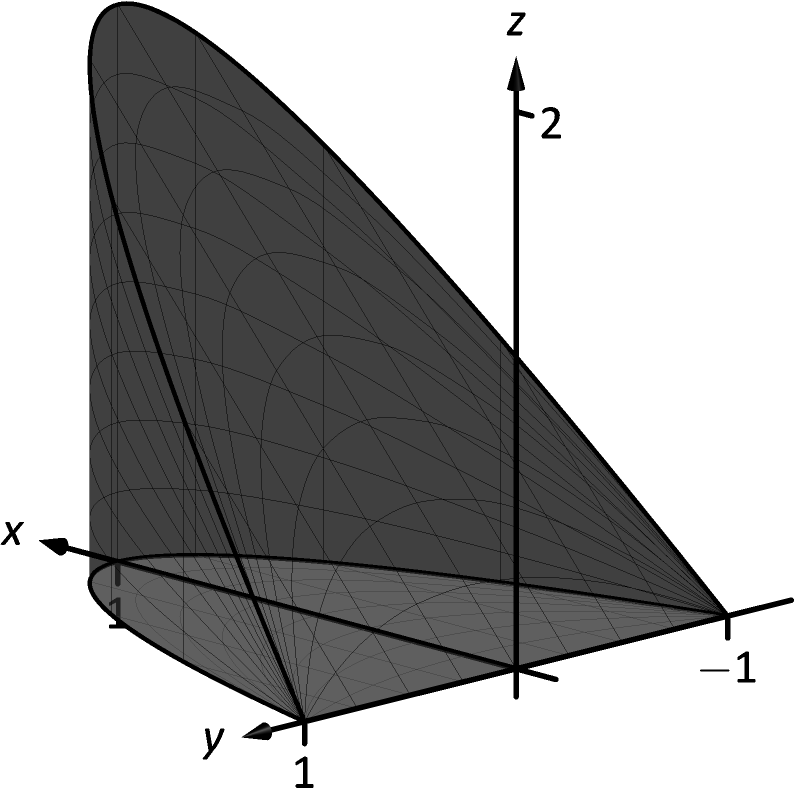
\includegraphics[width=\linewidth]{figdivthm_space2_3DBW}
\caption{A figure from the textbook with alt text:
\texttt{A wedge where 0<z<2x and 0<x<1-y².}
Make sure to grab and rotate the image.}
\label{threeDfig}
\end{figure}
It is not reasonable to describe a commutative diagram with fourteen cells
in at most 120 characters, nor can a short description convey the information
learned by rotating an image.
%More pertinent to the textbook, a defining feature is that the \PDF\ 
%includes many three dimensional figures that can be rotated
%in Adobe's \PDF\ viewer (see  for an example).
%
%{
%3Droll=1.320775024146522,
%3Dortho=0.004999999888241291,
%3Dc2c=0.6570873856544495 0.6839641332626343 0.31690558791160583,
%3Dcoo=-3.0739071369171143 -0.40104401111602783 58.57058334350586,
%3Droo=129.99999696026478}{.8\marginparwidth}{Surface z = x^2 + 2y^2 (Light blue). The vertical plane y = 2 cuts out the parabolic trace z = x^2 + 8 (heavy blue).}{figures/figpartialintro_3D}
%
On the other hand, there is no \emph{mathematical} problem with
having a longer description.
Accessibility guidelines suggest creating a short alt text pointing
to a longer description elsewhere.
I typically ignored that suggestion,
but tried to keep the alt text from getting too long.

A bigger problem arises in early chapters in the calculus sequence
when we ask students to verbally describe a graph,
as in \autoref{fig:calcprob}.
%
\begin{figure}
  \begin{center}
  \begin{tikzpicture}
  \begin{axis}[xmin=-2,xmax=2,ymin=-.1,ymax=1.6,width=\linewidth,
  axis x line=center,axis y line=center,axis equal image]
    \draw(-2,0.5)--(-1,1)circle(.04);
    \draw[fill=black](-1,0)circle(.04);
    \addplot[domain=-1:2]{.5*(x+1)*(x-1)^2};
  \end{axis}
  \end{tikzpicture}
  \end{center}
  \footnotesize
  Exercise: Describe this function, identifying limiting values, intercepts
  and their degree, critical and inflection points,
  and regions where the function is increasing, decreasing, and
  concave up or down.
%  \\
%  Model answer: this function has a domain of $-2\le x\le 2$.
%  From $(-2,0.5)$ is increases linearly toward a left hand limit at $(-1,1)$.
%  The function then has a jump discontinuity to be right continuous
%  at $(-1,0)$.
%  From that point, it increases to a local maximum near $(-0.4,0.6)$,
%  decreases through a $y$-intercept at $(0,0.5)$ to a local minimum at $(1,0)$
%  with even (possibly 2) degree.
%  Finally, it increases from that point to be near $(2,1.5)$.
%  The function is increasing on $[-2,-1]$; $[-1,-0.4]$; and $[1,2]$
%  and decreasing on $[-0.4,1]$.
%  It is concave up on $[0.2,2]$ and concave down on $[-1,0.2]$.
  \caption{\label{fig:calcprob}How do you write alt text for this exercise
  without giving away the answer?}
\end{figure}
I chose to describe the graph using various synonyms
(``the graph is a line from $(-2,0.5)$ to a hollow dot at $(-1,1)$, \dots''),
but acknowledge this is not an entirely satisfactory approach.

Many \PDF\ checkers do not recognize \PDF\ version 2.0 and
instead check the \PDF\ against version 1.7.
A critical distinction for us is that \PDF\ version 1.7 requires that
formulas include alt text.
We can accomplish this by uncommenting the \texttt{math/alt/use}
key in the \cs{DocumentMetadata} command.
This usually causes \PDF\ screen readers to read the alt text and
omit the more informative \MathML\ tags
(although there is a recent recommendation to the contrary at
\cite{bestPracticesURL}),
%\url{https://pdfa.org/resource/best-practice-guide-math-in-pdf/}
so I discourage its use
unless a document is being judged on its adherence to the 1.7 standard.

%A colleague uses the \texttt{rmarkdown} package,
%which has its own syntax for including graphics.
%This does not (yet?) allow specifying the alt text,
%which we therefore accomplish by using \verb|\setkeys{Gin}{alt={...}}|.
%Note that this setting will remain in effect until
%the next such command or when the group ends.

\section{Tables}

Tables need special consideration so that accessibility tools
are able to identify the headings that describe the data in the table.
But first, it should be emphasized that if the sole purpose of the table
is to arrange elements in a grid,
then it's not actually a table and probably shouldn't be tagged as such
(there are ways to tell the tagging code
``this doesn't need to be tagged as a table'',
but life will probably be easier if it's not a table to begin with).

To identify the headings in a particular tabular, I use
%\begin{verbatim}[setup-code=\small]
%\begin{verbatim}[\small]
\begin{verbatim}[\verbatimoptions]
\tagpdfsetup{
 table/header-rows={...},
 table/header-columns={...} }
\end{verbatim}
The default is an empty list specifying no header along that axis,
so that the most common occurrence of a single header row only needs
%\begin{verbatim}[setup-code=\small]
%\begin{verbatim}[\small]
\begin{verbatim}[\verbatimoptions]
\tagpdfsetup{table-header-rows={1}}
\end{verbatim}
and can omit the \texttt{table-header-columns}.
These declarations obey \TeX's grouping rules, so that a header
specification will last until the end of the current environment.

While \cs{multicolumn} is tagging ready, the same is not true for
a \cs{multirow} cell, which needs to have
%
%\newline
%{\small\ttfamily
%\cs{tagpdfsetup}%
%\tubbraced{table/multirow=\tubbraced{\meta{number of rows}}}}%
%
\begin{verbatim}[\verbatimoptions]
\tagpdfsetup{table/multirow={!<number of rows>}}
\end{verbatim}
at the beginning of the cell.

I should also note that the table interface
will likely change over the next few years.
Follow \texttt{texdoc latex-lab-table} for the details.


\section{Other package changes}

\begin{description}
\item[\texttt{titlesec}] Became \cs{@startsec}
(see \texttt{texdoc latex2e}, \S 6.8).
Another possibility is the new template mechanism
(see \texttt{texdoc latex-lab-sec-template}).
\item[\texttt{enumitem}] Became \texttt{enumext},
Also has a templating alternative
(see \texttt{texdoc blocks-doc}).
\item[\texttt{marginnote}] Became \texttt{marginalia}.
% \cs{marginpar} another possibility
\item[\texttt{media9}] Needed a deep dive into tagging internals
to properly tag the three dimensional images.
I wouldn't recommend that for
those getting started tagging their documents.
%It's also possible that the tagging of these items isn't quite correct,
%although the result is a well-tagged \acro{UA-2} \PDF.
\item[\texttt{beamer}] Became \texttt{ltx-talk}.
For more details, see my other article in this issue.%
\footnote{Not for the textbook, but as long as I'm mentioning package changes.}
\end{description}

\section{Checking the results}

Having resolved all possible errors,
I needed to verify that the result was indeed accessible.
The obvious first step is to ensure
a screen reader properly handles the document.
Unfortunately, when it comes to \PDF\ version 2.0,
the only currently viable \PDF\ readers are Adobe, Foxit, and Firefox,
while
the only currently viable screen readers to go with them are
\acro{NVDA} and \acro{JAWS} on Windows and Orca on
Linux\footnote{\url{https://tex.stackexchange.com/a/755945}}.
%\cite{screenReadersURL}.
I should also note that experienced users often use their screen readers
in a radically different manner than novice users,
so that this obvious first step may be necessary, but not sufficient.

Another approach to verifying accessibility is to verify that
the \PDF\ is indeed version 2.0,
and satisfies the \acro{UA-2} \PDF\ standard.
Unfortunately (again),
there are not many \PDF\ checkers that recognize version 2.0,
and many will apply version 1.7 standards to a version 2.0 document,
resulting in many claimed ``issues'' with a valid document%
% \cite{spuriousURL}.
\footnote{\url{https://github.com/latex3/tagging-project/discussions/categories/issues-with-accessibility-checkers-and-other-at-software}}.
%(for example, 1.7 but not 2.0 requires that formulas have alt text).
In the positive direction,
%\url{https://pdfa.org/accessible-math-in-pdf-finally/}
there are several (but currently only
five\footnote{and at least three of the five are different user interfaces
over the same validation profiles})
checkers that support \PDF\ version
2.0\footnote{\url{https://pdfa.org/accessible-math-in-pdf-finally}}.
% \cite{pdfCheckersURL}.
I have experience with
\veraPDF\footnote{\url{https://verapdf.org/}} and
\PDFix\footnote{\url{https://pdfix.net/}}.

The \LaTeX\ team uses \veraPDF\ to validate their documents,
so that using the same validation gives similar results
(this is usually good, but can be bad if they have overlooked an issue).
The main downside I find with \veraPDF\ is that
while it provides a \acro{GUI} to initiate a validation and see the results,
it reports the location of failed validation checks
as paths within the \PDF\ document, such as
%\begin{verbatim}[\verbatimoptions]
%root/
%  document[0]/
%  pages[14](925 0 obj PDPage)/
%  contentStream[0](926 0 obj
%    PDSemanticContentStream)/
%  content[124]{mcid:109}/
%  contentItem[0]{mcid:109}
%\end{verbatim}
\begin{verbatim}[\verbatimoptions]
root/
  document[0]/
  StructTreeRoot[0](5 0 obj PDStructTreeRoot)/
  K[0](22 0 obj SEDocument Document)/
  K[2130](24072 0 obj SESect figures)/
  K[71](102535 0 obj SEAside float)
\end{verbatim}
%Identifying the page is not sufficient to know which aspect
%is causing a failed validation.
\VeraPDF\ also has a command line version of the program,
allowing for faster (or even automated) checking of generated \PDF s.
\VeraPDF\ provides several profiles for checking \PDF s
at \cite{veraProfilesURL}.
For each profile, after a minute examining the Calculus textbook,
\veraPDF\ presents an \XML\ report that the text book is compliant,
as well as how many rules and checks it used for the profile,
summarized in \autoref{vera-report}.
\begin{table}
\centering
\caption{Successful validations examined}
\label{vera-report}
\begin{tabular}{l S[table-format=4] S[table-format=8,digit-group-size=4]}\toprule
Profile & {Rules} & {Checks} \\\midrule
\PDF/\acro{UA}-2 & 91 & 9051914 \\
\acro{ISO}-32005 & 1645 & 4200409 \\
\PDF/\acro{UA}-2 \& \acro{ISO}-32005 & 1727 & 12730361 \\
\acro{WCAG} 2.2 & 59 & 1186 \\
\acro{WCAG} 2.2 Dev & 23 & 0 \\  % semantic checks
\acro{WCAG} 2.2 Machine & 98 & 9053079 \\
\acro{WCAG} 2.2 Complete & 145 & 9053095 \\
\acro{WTPDF} 1.0 Accessibility & 1723 & 12730357 \\
\acro{WTPDF} 1.0 Reuse & 1710 & 11483386 \\\midrule
Combined & 1906 & 22305420 \\\bottomrule
\end{tabular}
\end{table}
(The \acro{WCAG} 2.2 Dev profile uses ``semantic'' checks
that only a human can verify.)
A default invocation of \veraPDF\ will give a report using the
\PDF/\acro{UA}-2 \& \acro{ISO}-32005 profile
and the two \acro{WTPDF} 1.0 profiles.
These do not need to be downloaded from \cite{veraProfilesURL}.
In my experience, a document that compiles successfully,
only uses supported packages,
and does not attempt strange constructions
will satisfy the validation profiles.

We can combine the profiles in
\autoref{vera-report}\footnote{\url{https://tex.stackexchange.com/a/763124}},
% \cite{combineProfilesURL},
although their overlap is unclear and the \acro{WCAG} profiles may move to
\acro{PDF4WCAG}\footnote{\url{https://pdf4wcag.com/}}\textsuperscript{,}%
\footnote{\url{https://github.com/latex3/tagging-project/discussions/1357\#discussioncomment-17086425}}.
% \cite{migrationURL}.

\PDFix\ uses a similar checker as \veraPDF, but it also provides a
graphical view of the \PDF\ in question, which better locates errors.
For example, \PDFix\ presents the \emph{same} validation error as in
\autoref{pdfixValError} (gray-scaled for print).
\begin{figure}
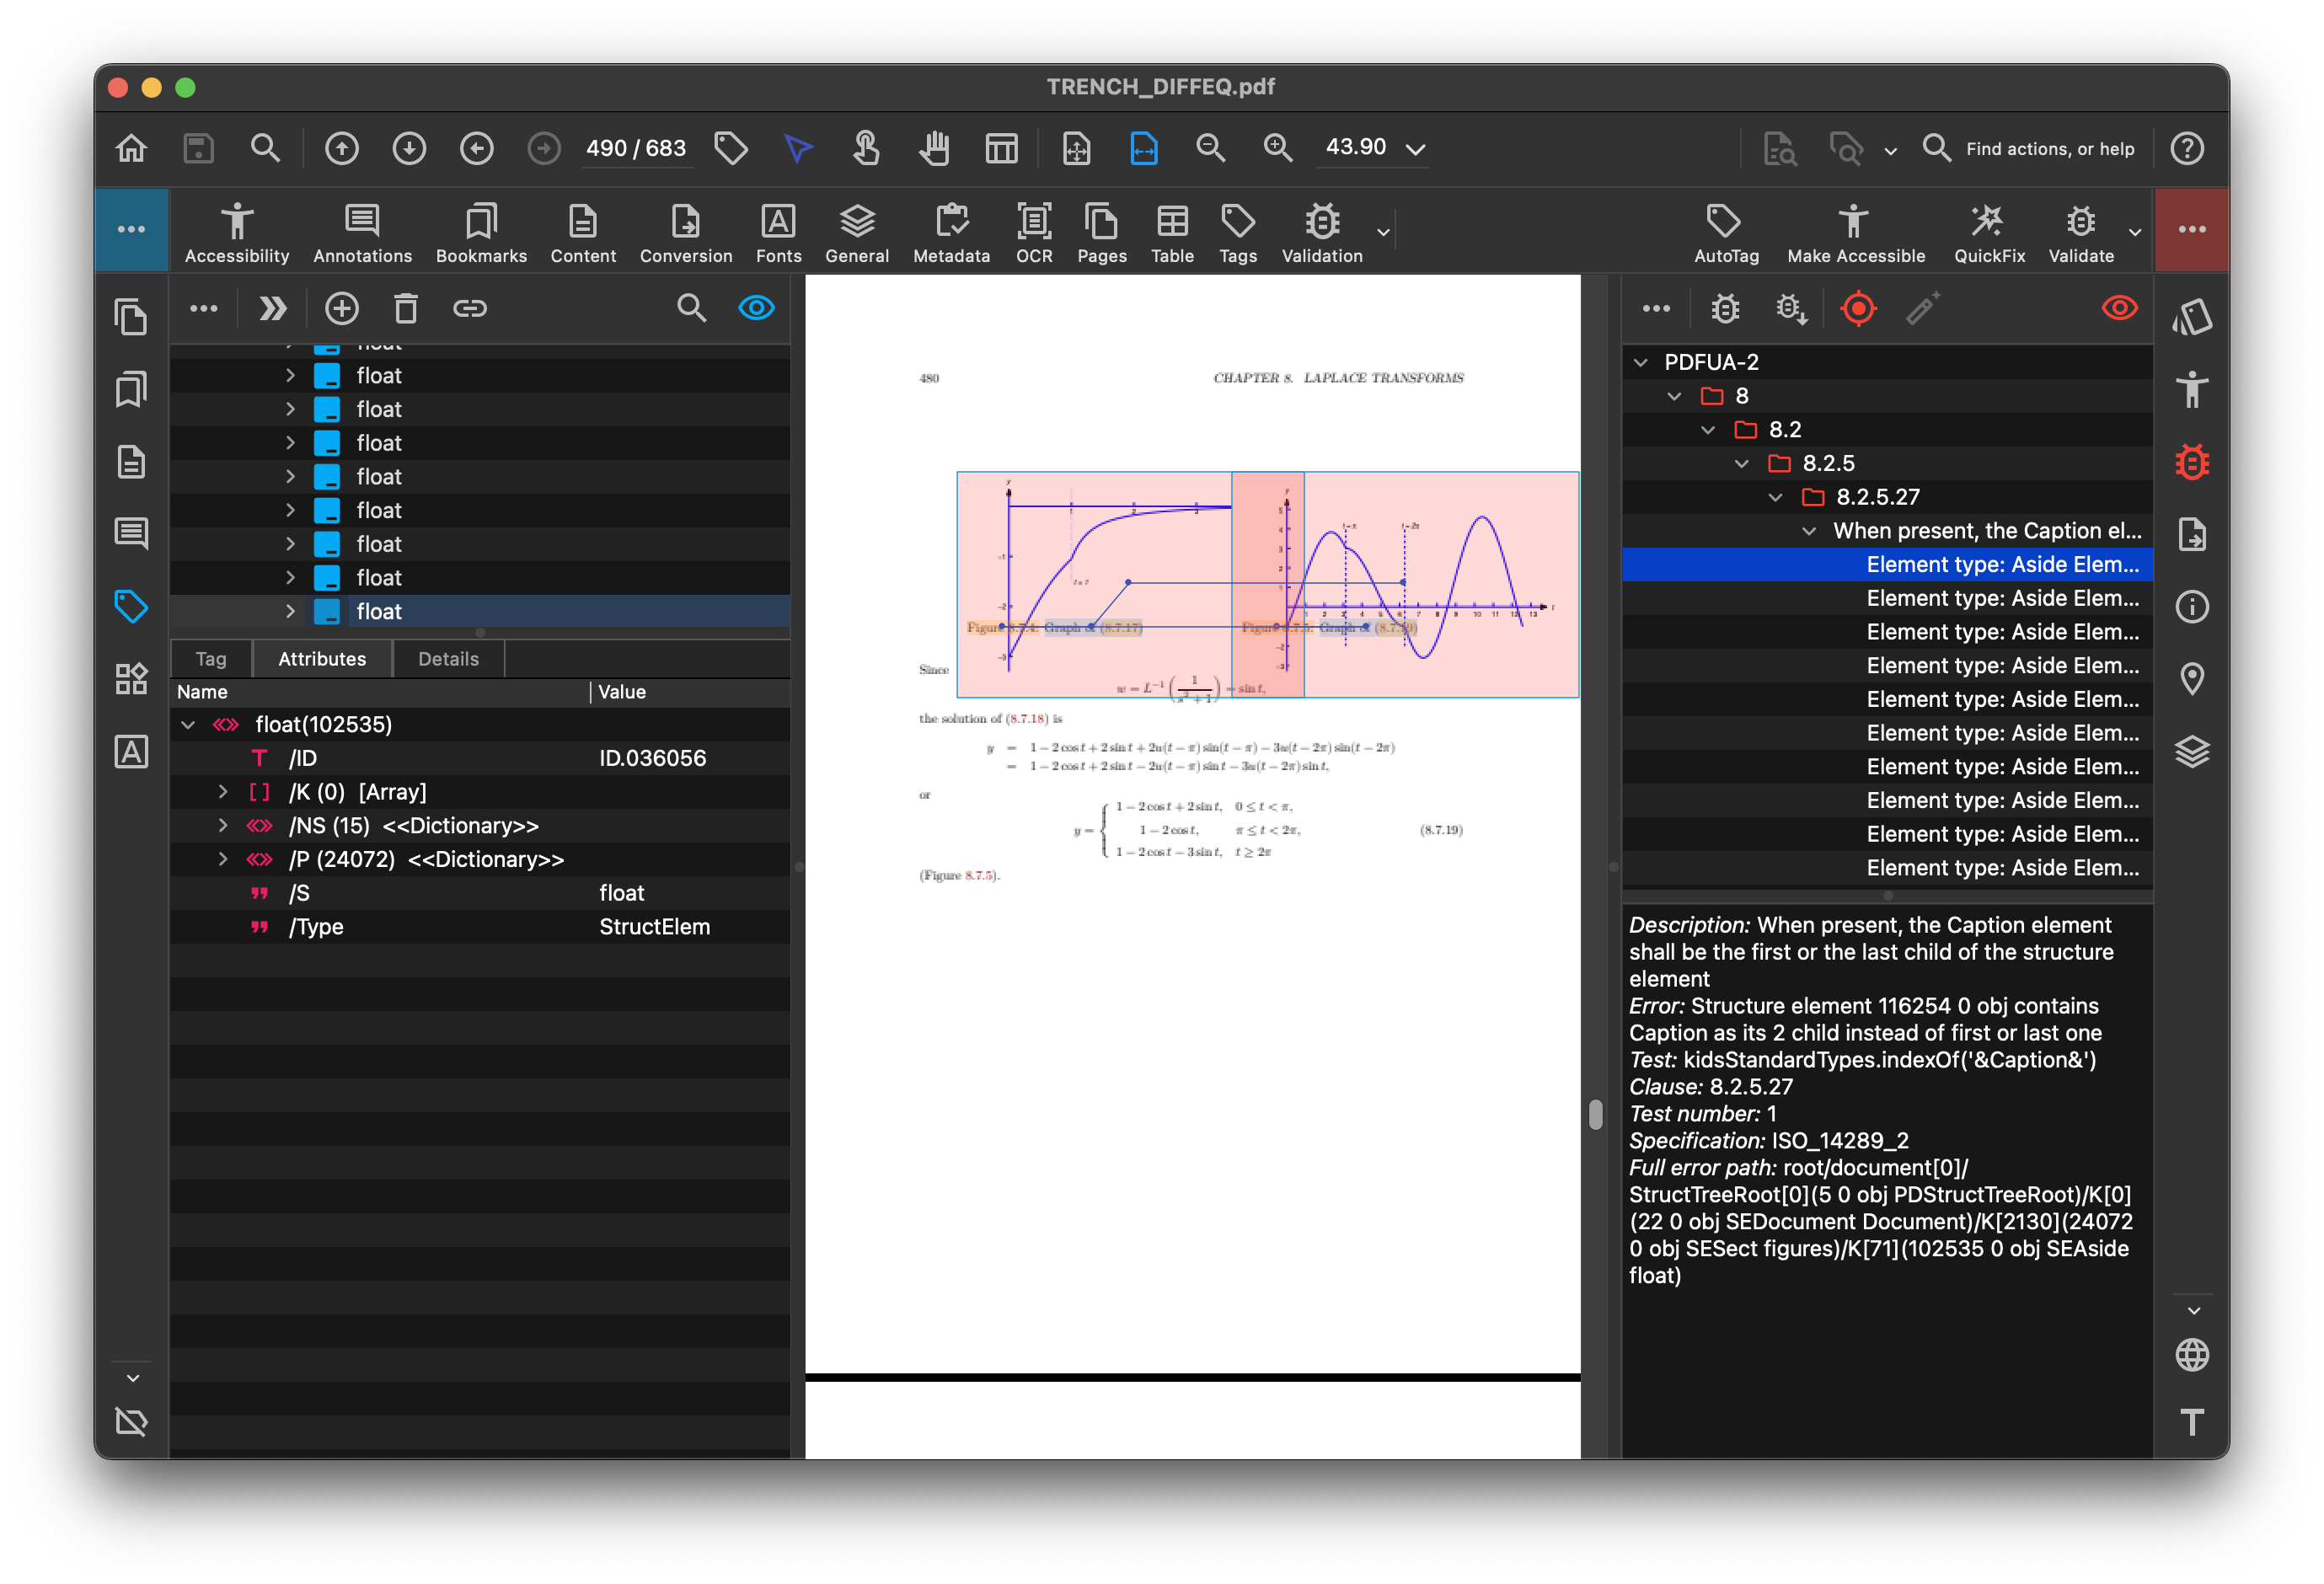
\includegraphics[width=\linewidth]{pdfixValError}
\caption{A \acro{UA}-2 validation error in \PDFix.}
\label{pdfixValError}
\end{figure}
\PDFix\ also allows navigating the tree structure of the \PDF,
making it possible to locate errors given by \veraPDF.
Additionally, \PDFix\ offers the profiles from \cite{veraProfilesURL}
without needing an additional installation.

My institution uses Ally to check \PDF s posted to our \acro{LMS}.
Ally is one of the aforementioned \PDF\ checkers that looks for version 1.7
and requires formulas to have alt text.
For this reason, I try to avoid posting the textbook to the \acro{LMS}.

Ally also requires that documents over two pages use
headings\footnote{\url{https://help.anthology.com/ally-lms/en/administrators/ally-accessibility-checklist.html}}.
% \cite{allyChecksURL}.
I normally accomplish this with \cs{section} commands,
but if a document does not otherwise have them,
it is possible to have the title also serve as a
heading\footnote{\url{https://tex.stackexchange.com/a/758805}}.
% \cite{titleHeadingURL}.

For shorter documents, I can also examine the tagging structure
of a \PDF\ by using the command line tool \texttt{show-pdf-tags}
or \acro{ngPDF}\footnote{\url{https://ngpdf.com/}}.

\section{Other textbooks and lessons learned}

Since converting the calculus textbook to be accessible,
I have also converted a linear algebra
textbook\footnote{\url{https://github.com/teepeemm/LinearAlgebra}}
and a differential equations
textbook\footnote{\url{https://github.com/teepeemm/trenchDEs}}
to both be accessible.

The most work involved is when someone used manual formatting
instead of \LaTeX\ defaults\footnote{\cs{over} wasn't all that fun, either}.
Typing \verb|1. ... 2. ... 3.| instead of using
an \tubbraced{enumerate} environment may yield a similar looking \PDF,
but the manually formatted version cannot be properly tagged.
This requires revisions to replace the manual formatting
with the \LaTeX\ defaults, and possibly more work
to make the defaults resemble the original manually formatted version.

On the other hand,
replacing manual formatting with \LaTeX\ defaults creates
a more readable, more maintainable, and more accessible document.
I would argue that the one time cost of doing so
is well worth the few hours required for the result.

Accessible \PDF s require more computing power to create.
\begin{table}
\caption{Factor by which various statistics increase
for compiling tagged textbooks.}
\label{results}
\centering
\begin{tabular}{lS[table-format=2(1),uncertainty-mode=separate]}\toprule
Statistic & Factor \\\midrule
Time & 10(3) \\
\acro{RAM} & 6(2) \\
Output size & 2(1) \\
strings & 11(4)\\
hash & 10(4)\\\bottomrule
\end{tabular}
\end{table}
\autoref{results} reports the factor
by which various computational statistics increase for the textbooks,
along with the rather large uncertainty of these numbers.
My guess is that the uncertainty depends on how complicated the original
textbook is: a complicated project starts with large statistics,
so that adding tagging increases the statistics by not as much relatively.
The final two entries of the table relate
how much memory the compilation process requires.
This originally resulted in fatal compilation errors that
\TeX\ exceeded its capacity for
the \texttt{number of strings} or the \texttt{hash size},
requiring me to modify the compilation
command\footnote{\url{https://tex.stackexchange.com/a/741777/}}.
% \cite{moreMemoryURL}.

I have encountered some misconceptions during this process.
Some people think that \PDF s, especially those produced by \LaTeX,
are inherently inaccessible.
This is usually because they are not using the techniques from this article,
or they are not using (one of the few) screen readers
that can properly handle the output.
A separate misconception is that inaccessibilities in a \LaTeX\ \PDF\ must
be remediated elsewhere (usually in Adobe Pro),
a time intensive and costly process.
These people often do not realize that transforming
a tex file into a \PDF\ means we have the ability
to remediate as we create the \PDF.
Nor do they realize that the goal of the \LaTeX\ team
is to obviate any remediation requirement.

As a final remark, I have collected the advice from this article
into a GitHub repository at \cite{accessibleURL}.

\iffalse

This is an example article for \TUB, linked from
\url{https://tug.org/TUGboat/location.html}.

\section{Basic packages and hyperlinks}

The standard \texttt{graphicx} and \texttt{xcolor} packages work fine
for image and color handling, respectively, as does the
\texttt{hyperref} package for active urls. \TUB\ is produced using
\PDF\ files exclusively, but conversion from \DVI\ is fine and supported.

Please use the standard \cs{url} command for urls:
\begin{verbatim}
\url{https://some/url} % yes
\end{verbatim}
For \TUB, we prefer not to print the `\texttt{https://}', but to include
the protocol in other cases, so we usually do \verb|\def\url{\tburl}|,
which takes care of that, while keeping the source using the standard
\cs{url} command.

In any case, please do \emph{not} hide hyperlinks via \cs{href}, as in:
\begin{verbatim}
\href{https://some/url}{some text} % no!
\end{verbatim}
When printed on paper, the url will not be visible and readers will
not know it exists.

\section{Abbreviation macros and typing}

The \texttt{ltugboat} class provides many abbreviation commands; here
are a few of the most common:

% verbatim blocks are often better in \small
%\begin{verbatim}[\small]
\begin{verbatim}
\AllTeX \AMS \BibTeX \Cplusplus \CTAN \DVI
\HTML \LaTeXe \macOS \MathML \MF \PDF \PS
\TUB \TUG \tug \WEB \XeLaTeX \XeTeX \XML
\end{verbatim}

A few other typing conventions:

\begin{itemize}
\item For an em-dash with our spacing (preferred to \verb|---|):
\cs{Dash}, with output\Dash like this.

\item For initialisms in all caps:
\verb|\acro{FRED}|,\\ with output: \acro{FRED}.

\item A literal control sequence:
\verb|\cs{fred}|,\\ with output: \cs{fred}.

\item A syntactic metavariable:
\verb|\meta{fred}|,\\ with output: \meta{fred}.

\item A title:
\verb|\titleref{Book of Fred}|,\\ with output: \titleref{Book of Fred}.
\end{itemize}

We recommend using \cs{begin}\tubbraced{verbatim}\texttt{[\cs{small}] ...}
\cs{end}\tubbraced{verbatim} for code blocks, since we prefer not to
colorize code when printed. But if you want to have some font changes,
our recommended settings for the \texttt{listings} package are in the
\texttt{ltubguid} manual mentioned below.

Please put punctuation outside quotes, ``like this'', unless the
punctuation is actually part of the quoted material.

Also, please put punctuation after footnotes.

\section{Figures}

For \TUB, the standard \texttt{figure} environment produces a
column-width figure; this is desirable when at all possible. The
\texttt{figure*} environment produces a full-width (across both columns)
figure when needed. Analogously for \texttt{table} and \texttt{table*}.

Please put captions below figures, but above tables.

Don't worry overmuch about figure placements, as they will likely change
with editing.

\section{References}

For references to other issues of \TUB, please use the format
\textsl{volno}:\textsl{issno}, e.g., ``\TUB\ 32:1''.

The primary \TUB\ style documentation is the \texttt{ltubguid} manual,
available online at \tbsurl{ctan.org/pkg/tugboat} or locally with
\texttt{texdoc tugboat}. For general \CTAN\ package references, we
recommend that form, using \texttt{/pkg/}. If you need to refer to a
specific file on \CTAN, use:\\
\texttt{https://mirror.ctan.org/\textsl{path}}

We recommend using \BibTeX\ (but don't require it), with the
\texttt{tugboat} \BibTeX\ style. The \texttt{biblio} directory on \CTAN,
\tbsurl{ctan.org/pkg/biblio}, provides files \texttt{tugboat.bib} with a
complete bibliography of \TUB, \texttt{texbook3.bib} with many common
\TeX-related books and articles, and plenty more.

Email \verb|tugboat@tug.org| with any questions.

\fi

\bibliographystyle{tugboat} % tugboat's bibtex style
%\nocite{book-minimal}       % make the example bibliography non-empty
\bibliography{references,tugboat}
%\bibliography{xampl}        % xampl.bib comes with bibtex

\makesignature
\end{document}
